% ===========================================================
%  Лекция 12. Хроматический многочлен
% ===========================================================

\chapter{Лекция 12. Хроматический многочлен}

\begin{defn}{Хроматический многочлен}{chromatic-polynomial}
Пусть $G(V, E)$~--- граф. \textbf{Хроматический многочлен} графа $G$:
\[
  P_G\colon \mathbb{N}_0 \to \mathbb{N}_0, \qquad
  P_G(t) = a_1 t + a_2 t^2 + \ldots + a_n t^n,
\]
т.\,е.\ это многочлен, значение которого $P_G(k)$ равно числу правильных раскрасок $G$ в $k$ цветов ($\forall\, k \in \mathbb{N}_0$).
\end{defn}

\textbf{Примеры:}
\begin{enumerate}
  \item Пустой граф ($n$ изолированных вершин): $P_G(t) = t^n$ ---
        каждая вершина красится независимо любым из $t$ цветов.
  \item $K_n$: $P_{K_n}(t) = t(t-1)(t-2)\cdots(t-(n-1))$ --- красим
        вершины по очереди, каждая обязана отличаться от всех
        предыдущих.
  \item Дерево $T_n$ ($n$ вершин): $P_{T_n}(t) = t(t-1)^{n-1}$ ---
        красим от корня: корень $t$ способами, каждую следующую вершину
        (по мере удаления от корня) --- $t - 1$ способами, лишь бы она
        отличалась от единственного уже покрашенного соседа (родителя).
\end{enumerate}

Иллюстрация на двух деревьях с $n = 4$ (показана одна из правильных
раскрасок в 2 цвета):

\grfig[0.4]{figures/p26-example-1.pdf}{Путь $P_4$: $P(t) = t(t-1)^3$; в 2 цвета --- ровно 2 раскраски}
\grfig[0.4]{figures/p26-example-2.pdf}{Звезда: тоже $P(t) = t(t-1)^3$ --- дерево с тем же $n$}

Заметим: путь и звезда --- \emph{разные} графы с \emph{одинаковым}
хроматическим многочленом (см.~свойство 4 ниже).

\medskip
\textbf{Тривиальные свойства} (с обоснованиями):
\begin{enumerate}[label=\arabic*)]
  \setcounter{enumi}{-1}
  \item $P_G$~--- многочлен. \textit{Почему:} сгруппируем раскраски по
        числу $i$ реально использованных цветов: если $\alpha_i$ ---
        число разбиений $V$ на $i$ непустых независимых (попарно
        несмежных внутри) множеств, то
        $P_G(t) = \sum_{i} \alpha_i \cdot t(t-1)\cdots(t-i+1)$ ---
        выбираем, какие именно $i$ из $t$ цветов достанутся классам
        разбиения. Это конечная сумма многочленов.
  \item $\deg(P_G) = |V|$. \textit{Почему:} старшее слагаемое в сумме
        выше отвечает $i = n$ (все вершины разных цветов, $\alpha_n = 1$)
        и равно $t(t-1)\cdots(t-n+1)$ --- многочлен степени $n$.
  \item $P_G(0) = 0$ для $\forall\, G$ т.\,ч.\ $|V| > 0$:
        в $0$ цветов нельзя раскрасить даже одну вершину.
  \item $P_G(t) = t^k \cdot g(t)$, где $g(0) \neq 0$, $k$~--- число
        компонент связности графа $G$. \textit{Почему:} компоненты
        красятся независимо, поэтому $P_G$ --- произведение многочленов
        компонент, и каждый сомножитель делится на $t$ ровно один раз.
  \item $G$ по $P_G$ не восстанавливается однозначно.
        \textit{Контрпример:} все деревья на $n$ вершинах имеют один и
        тот же многочлен $t(t-1)^{n-1}$, но при $n \ge 4$ дерево не
        единственно (путь $P_4$ и звезда на рисунках выше).
  \item $a_n = 1$ (старший коэффициент) --- см.~обоснование свойства 1.
  \item $\forall\, 1 \leq i \leq n-1\colon a_i \cdot a_{i+1} \leq 0$
        (знакочередование). \textit{Идея:} индукция по числу рёбер с
        теоремой о редукции в форме
        $P_G = P_{G \setminus e} - P_{G/e}$: у $P_{G\setminus e}$
        и $P_{G/e}$ знаки чередуются по предположению, степени
        отличаются на $1$, и при вычитании чередование сохраняется.
  \item $|E_G| > 0 \;\Rightarrow\; P_G(1) = 0$: при одном цвете концы
        любого ребра совпадут по цвету. Более точно,
        $P_G(t) = (t-1)^d \cdot g(t)$, где $g(1) \neq 0$, $d$~--- число
        блоков (компонент вершинной двусвязности) в $G$.
\end{enumerate}

\subsection*{Как найти $P_G$?}

\begin{statement}{Теорема о редукции}{reduction-theorem}
Пусть $G(V, E)$, и $u, v \in V$~--- не смежные вершины. Тогда:
\[
  P_G(t) = P_{G \vee uv}(t) + P_{G * uv}(t),
\]
где $G \vee uv$~--- граф с добавленным ребром $uv$ (приближаем к полному), а $G * uv$~--- граф со стянутыми вершинами $u$ и $v$.
\end{statement}

\begin{proof}
Разобьём все правильные раскраски $G$ в $t$ цветов на два класса по
тому, как покрашены $u$ и $v$ (они не смежны, поэтому возможно и то,
и другое):
\begin{itemize}
  \item \textbf{цвета $u$ и $v$ различны} --- такие раскраски взаимно
        однозначно соответствуют правильным раскраскам графа
        $G \vee uv$: добавленное ребро $uv$ как раз и требует
        различия цветов, остальные ограничения совпадают;
  \item \textbf{цвета $u$ и $v$ совпадают} --- такие раскраски взаимно
        однозначно соответствуют правильным раскраскам графа $G * uv$:
        склеенная вершина получает этот общий цвет, и её смежности ---
        объединение смежностей $u$ и $v$.
\end{itemize}
Классы не пересекаются и исчерпывают все раскраски, поэтому
$P_G = P_{G \vee uv} + P_{G * uv}$.
\end{proof}

Иллюстрация: $u$ и $v$ не смежны в $G$; слева направо --- $G$,
$G \vee uv$ (зелёное ребро добавлено), $G * uv$ (вершины склеены):

\begin{center}\begin{tabular}{ccc}
\shortstack{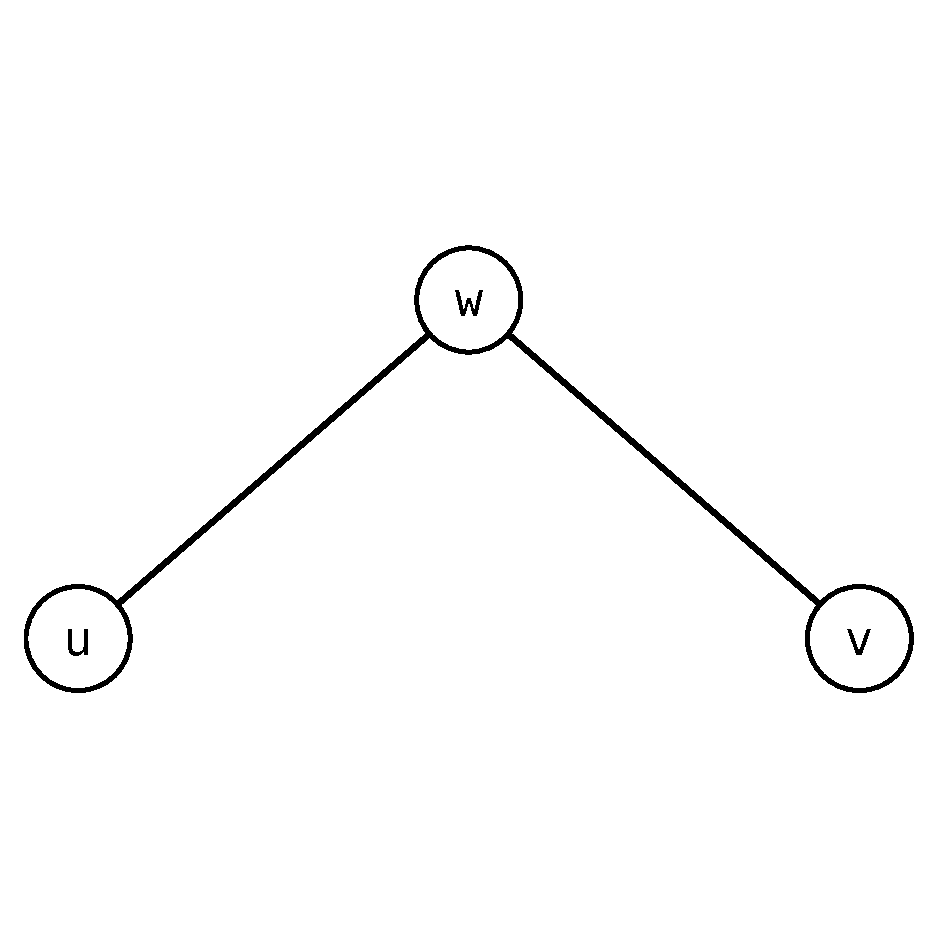
\includegraphics[width=0.26\textwidth]{figures/p26-red-0.pdf}\\[2pt]{\scriptsize $G$: путь $u$--$w$--$v$}} &
\shortstack{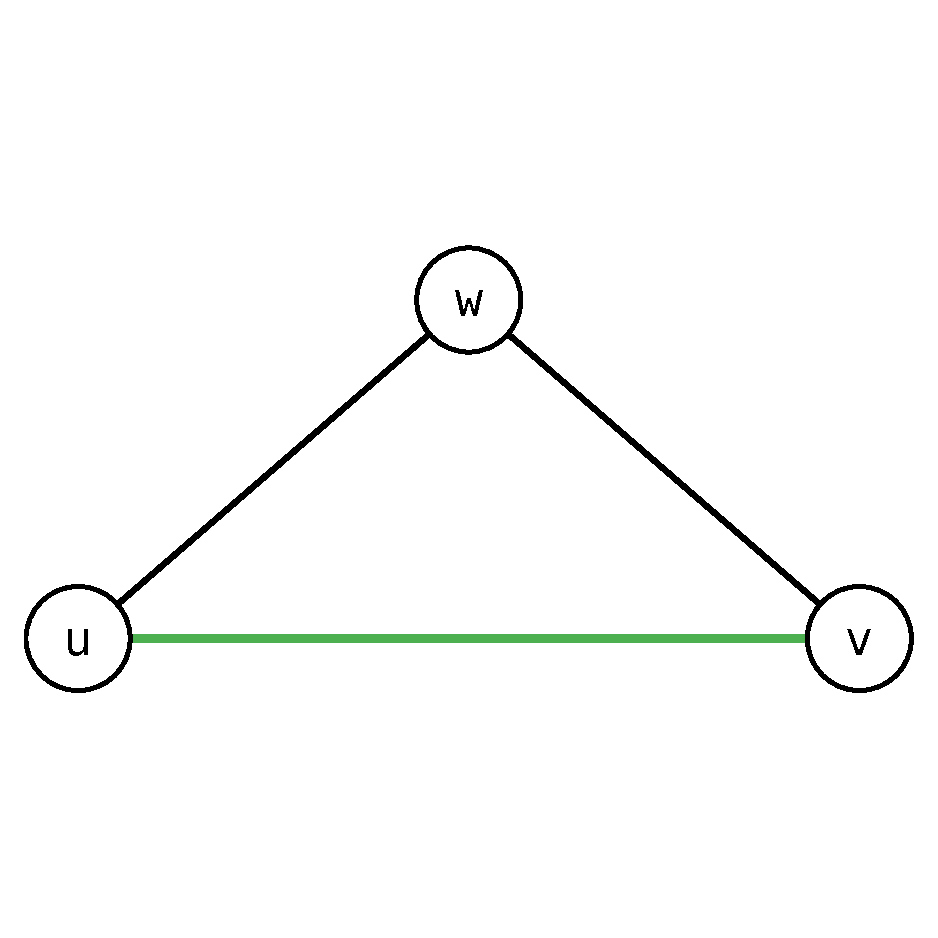
\includegraphics[width=0.26\textwidth]{figures/p26-red-1.pdf}\\[2pt]{\scriptsize $G \vee uv$: треугольник}} &
\shortstack{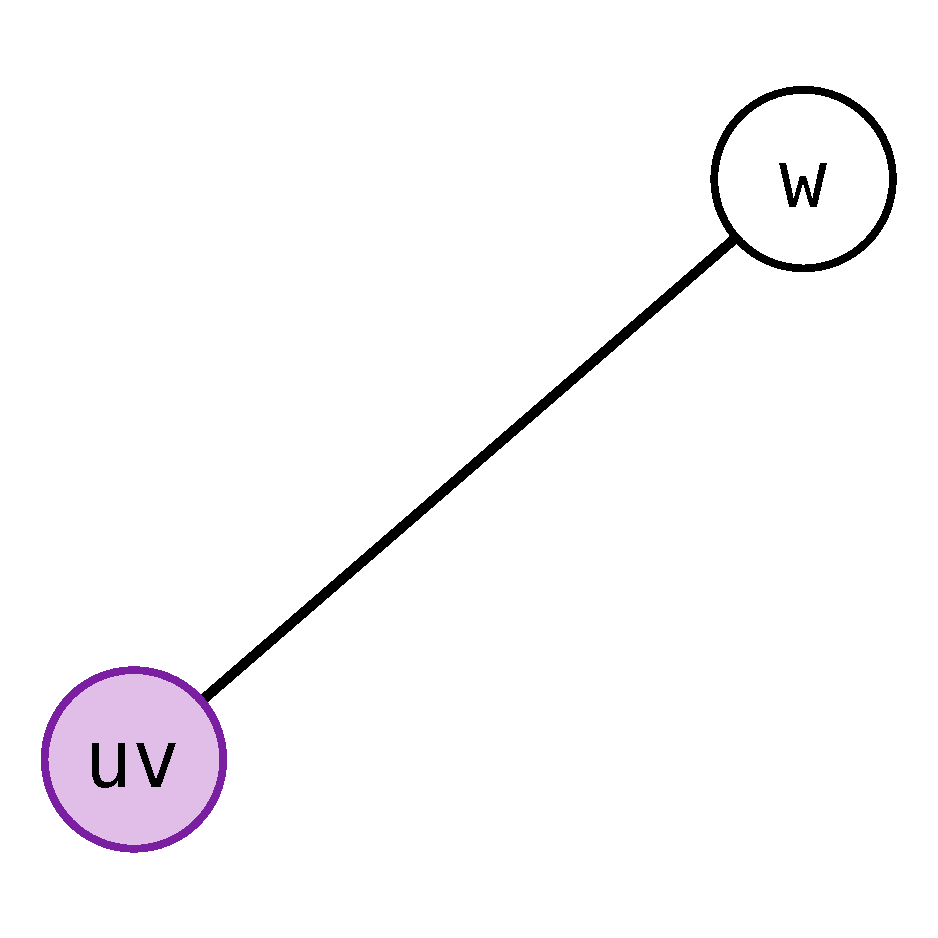
\includegraphics[width=0.26\textwidth]{figures/p26-red-2.pdf}\\[2pt]{\scriptsize $G * uv$: ребро}} \\
\end{tabular}\end{center}

\noindent\textbf{Мини-пример} (проверка теоремы). Для пути
$G = u$--$w$--$v$ на рисунке: $G \vee uv = K_3$, $G * uv = K_2$,
\[
  P_{G \vee uv} + P_{G * uv} = t(t-1)(t-2) + t(t-1) = t(t-1)^2
\]
--- в точности $P_{T_3}(t) = t(t-1)^2$ по формуле для дерева. $\checkmark$

\medskip
\textbf{Следствие.} Если $\exists\, e = uv$ (смежные), то:
\[
  P_G(t) = P_{G \setminus e}(t) - P_{G * uv}(t).
\]
\textit{Почему:} применим теорему к графу $G \setminus e$ (в нём $u, v$
уже не смежны): $P_{G \setminus e} = P_{(G\setminus e) \vee uv} +
P_{(G \setminus e) * uv} = P_G + P_{G * uv}$, и перенесём слагаемое.

\medskip
\textbf{Пример:} Цикл $C_n$:
\[
  P_{C_n}(t) = (t-1)^n + (-1)^n (t-1).
\]

\begin{proof}
Воспользуемся теоремой об удалении и стягивании: для любого ребра $e=uv$
\[
  P_G(t) = P_{G\setminus e}(t) - P_{G/e}(t),
\]
где $G\setminus e$ --- граф с удалённым ребром, а $G/e$ --- граф со
стянутым ребром (вершины $u$ и $v$ отождествлены). Понадобится также
хроматический многочлен простого пути (дерева) на $n$ вершинах:
$P_{T_n}(t)=t(t-1)^{n-1}$ (первую вершину красим $t$ способами, каждую
следующую --- $t-1$ способами, лишь бы она отличалась от предыдущей).

\textbf{База ($n=3$).} $C_3=K_3$, поэтому $P_{C_3}(t)=t(t-1)(t-2)$.
Проверим формулу:
\[
  (t-1)^3+(-1)^3(t-1)=(t-1)\bigl[(t-1)^2-1\bigr]=(t-1)(t^2-2t)=t(t-1)(t-2).
\]

\textbf{Переход.} Возьмём в цикле $C_n$ произвольное ребро $e=uv$. Его удаление
размыкает цикл в путь: $C_n\setminus e=T_n$, поэтому
$P_{C_n\setminus e}(t)=t(t-1)^{n-1}$. Стягивание ребра $e$ склеивает $u$ и $v$
и превращает цикл из $n$ вершин в цикл из $n-1$ вершины: $C_n/e=C_{n-1}$.
По теореме об удалении и стягивании
\[
  P_{C_n}(t)=t(t-1)^{n-1}-P_{C_{n-1}}(t).
\]
Подставляя предположение индукции
$P_{C_{n-1}}(t)=(t-1)^{n-1}+(-1)^{n-1}(t-1)$, получаем
\[
  P_{C_n}(t)=t(t-1)^{n-1}-(t-1)^{n-1}-(-1)^{n-1}(t-1)
           =(t-1)^{n-1}(t-1)+(-1)^{n}(t-1),
\]
то есть $P_{C_n}(t)=(t-1)^n+(-1)^n(t-1)$, что и требовалось.
\end{proof}

\subsection*{Теорема о разделяющей клике}

\begin{lemma}{Лемма 1 (висячая вершина)}{separating-clique-1}
Если в графе $G$ есть висячая вершина $u$, соединённая с подграфом $G_1$, то:
\[
  P_G(t) = P_{G_1}(t) \cdot (t-1).
\]
\grfig{figures/p27-lemma1.pdf}{Лемма 1: висячая вершина -> P\_G = P\_\{G1\}.(t-1)}
\end{lemma}

\begin{proof}
Сначала правильно красим $G_1$ --- $P_{G_1}(t)$ способами. У вершины $u$
ровно один сосед, и какой бы цвет он ни получил, для $u$ остаётся
$t - 1$ допустимых цветов; выбор независим от остального. По правилу
произведения $P_G(t) = P_{G_1}(t)(t-1)$.
\end{proof}

\begin{lemma}{Лемма 2 (дерево $T_{n+1}$)}{separating-clique-2}
Если к подграфу $G_1$ присоединено дерево $T_{n+1}$ (через одну вершину), то:
\[
  P_G(t) = P_{G_1}(t) \cdot (t-1)^n.
\]
\grfig{figures/p27-lemma2.pdf}{Лемма 2: дерево T\_\{n+1\} -> P\_G = P\_\{G1\}.(t-1)\^{}n}
\end{lemma}

\begin{proof}
Дерево $T_{n+1}$ имеет $n + 1$ вершину (одна из них --- общая с $G_1$)
и $n$ рёбер. Присоединяем его вершины по одной, начиная от общей вершины
и удаляясь по дереву: каждая новая вершина --- висячая относительно уже
покрашенной части, и по лемме~1 даёт множитель $(t-1)$. Всего $n$ новых
вершин: $P_G = P_{G_1} \cdot (t-1)^n$.
\end{proof}

\begin{lemma}{Лемма 3 (вершина при ребре)}{separating-clique-3}
Если вершина $u$ присоединена к $G_1$ рёбрами к \emph{обоим концам}
некоторого ребра $vw \in G_1$ (т.\,е.\ через клику $K_2$), то:
\[
  P_G(t) = P_{G_1}(t) \cdot (t-2).
\]
\grfig{figures/p27-lemma3.pdf}{Лемма 3: вершина при ребре -> P\_G = P\_\{G1\}.(t-2)}
\end{lemma}

\begin{proof}
В любой правильной раскраске $G_1$ концы ребра $vw$ покрашены в
\emph{два различных} цвета. Вершине $u$ запрещены ровно эти два цвета,
остаётся $t - 2$ вариантов --- независимо от того, какая именно
раскраска $G_1$ выбрана.
\end{proof}

\begin{lemma}{Лемма 4 (вершина при $K_n$)}{separating-clique-4}
Если вершина $u$ с $\deg u = n$ присоединена к подграфу $G_1$ через $K_n$
(все $n$ соседей $u$ попарно смежны в $G_1$), то:
\[
  P_G(t) = P_{G_1}(t) \cdot (t - n).
\]
\grfig{figures/p27-lemma4.pdf}{Лемма 4: вершина при K\_n -> P\_G = P\_\{G1\}.(t-n)}
\end{lemma}

\begin{proof}
Соседи $u$ образуют клику, поэтому в любой правильной раскраске $G_1$
они покрашены в $n$ \emph{попарно различных} цветов. Для $u$ запрещены
ровно $n$ цветов --- остаётся $t - n$ вариантов. Леммы 1 и 3 ---
частные случаи при $n = 1$ и $n = 2$.
\end{proof}

\begin{lemma}{Лемма 5 (комбинация подвесок)}{separating-clique-5}
Если к $G_1$ присоединены висячая вершина и вершина при ребре
(как на рисунке), множители перемножаются:
\[
  P_G(t) = P_{G_1}(t) \cdot (t-1)(t-2).
\]
\grfig{figures/p27-lemma5.pdf}{Лемма 5: висячая вершина + вершина при ребре}
\end{lemma}

\begin{proof}
Применяем леммы по очереди: сначала к $G' = G$ без висячей вершины
$5$ --- по лемме~3 (вершина $6$ при ребре $3$--$4$) имеем
$P_{G'} = P_{G_1}(t-2)$; затем возвращаем висячую вершину $5$ --- по
лемме~1 получаем $P_G = P_{G'}(t-1) = P_{G_1}(t-1)(t-2)$. Порядок
применения не важен: каждая подвеска даёт свой множитель независимо.
\end{proof}

\begin{lemma}{Лемма 6 (общая, разделяющая $K_n$)}{separating-clique-6}
Если граф $G$ разделяется кликой $K_n$ на подграфы $G_1$ и $G_2$
(т.\,е.\ $G = G_1 \cup G_2$, $G_1 \cap G_2 = K_n$), то:
\[
  P_G(t) = \frac{P_{G_1}(t) \cdot P_{G_2}(t)}{P_{K_n}(t)}.
\]
\grfig{figures/p27-lemma6.pdf}{Лемма 6: общая, K\_n -> P\_G = P\_\{G1\}.P\_\{G2\}/P\_\{K\_n\}}
\end{lemma}

\begin{proof}
Ключевое наблюдение: \emph{число продолжений} фиксированной правильной
раскраски клики $K_n$ до правильной раскраски всего $G_1$ не зависит
от того, какая именно раскраска клики выбрана. Действительно, любые две
правильные раскраски $K_n$ ($n$ попарно различных цветов) переводятся
друг в друга перестановкой цветов, а перестановка цветов --- биекция
на множестве продолжений. Поэтому продолжений ровно
$P_{G_1}(t) / P_{K_n}(t)$ (всего раскрасок $G_1$, делённое на число
раскрасок клики); аналогично для $G_2$.

Раскраска $G$ --- это раскраска клики ($P_{K_n}(t)$ способов) плюс
независимые продолжения на $G_1$ и на $G_2$ (общих вершин вне клики
нет, рёбер между $G_1 \setminus K_n$ и $G_2 \setminus K_n$ нет):
\[
  P_G = P_{K_n} \cdot \frac{P_{G_1}}{P_{K_n}} \cdot \frac{P_{G_2}}{P_{K_n}}
      = \frac{P_{G_1} \cdot P_{G_2}}{P_{K_n}}.
\]
Леммы 1--5 --- частные случаи (например, лемма 4: $G_2 = K_{n+1}$,
$P_{G_2}/P_{K_n} = t - n$).
\end{proof}

\subsection*{Рёберная раскраска}

\begin{defn}{Правильная рёберная раскраска}{proper-edge-coloring}
Рёберная раскраска графа называется \textbf{правильной}, если $\forall\, e_1, e_2 \in E$, имеющие общую вершину, окрашены в разные цвета.
\end{defn}

\begin{defn}{Хроматически двойственный граф}{chromatic-dual}
Пусть $G(V, E)$. \textbf{Хроматически двойственный} граф $G_\chi(V_\chi, E_\chi)$ строится так:
\begin{enumerate}
  \item $V_\chi = E$ \quad (вершины $G_\chi$~--- это рёбра $G$);
  \item $\hat{u}, \hat{v} \in V_\chi$: $\exists\, \hat{e} = \hat{u}\hat{v} \;\Leftrightarrow\;$ рёбра $u, v \in E$ имеют общую вершину в $G$.
\end{enumerate}
Правильные \emph{рёберные} раскраски $G$ --- это в точности правильные
\emph{вершинные} раскраски $G_\chi$, поэтому рёберное хроматическое
число $\chi'(G) = \chi(G_\chi)$.
\end{defn}

\textbf{Пример} (рис.~p28-example-1 $\to$ p28-chromatic-dual):

Граф $G$: вершины $A, B, C, D, E$; рёбра $AB, BC, CA, CD, BE, DB$.

Хроматически двойственный $G_\chi$: вершины $AB, BC, CA, CD, BE, DB$; рёбра~--- пары, имеющие общую вершину в $G$.

\grfig{figures/p28-example-1.pdf}{Рёберная раскраска: исходный граф G (A,B,C,D,E)}
\grfig{figures/p28-chromatic-dual.pdf}{Хром. двойственный G\_χ (AB,BC,CA,CD,BE,DB)}

Заметим: четыре ребра $AB, BC, BE, DB$ инцидентны вершине $B$
($\deg B = 4$), поэтому в $G_\chi$ они образуют клику $K_4$ --- по
лемме о клике $\chi'(G) = \chi(G_\chi) \ge 4$.

\subsection*{Оценки на хроматическое число}

Обозначим $\Delta(G) = \max_{v \in V} \deg(v)$.

\begin{statement}{Жадная оценка}{greedy-bound}
\[
  \chi(G) \leq \Delta(G) + 1.
\]
\end{statement}

\begin{proof}
Красим вершины в произвольном порядке, выделив $\Delta + 1$ цветов.
Когда очередь доходит до вершины $v$, покрашено не более $\deg(v) \le
\Delta$ её соседей --- они запрещают не более $\Delta$ цветов, и хотя
бы один из $\Delta + 1$ цветов свободен. Оценка точна: для $K_n$ и для
нечётных циклов достигается равенство (теорема Брукса утверждает, что
во всех остальных связных графах $\chi \le \Delta$).
\end{proof}

\begin{statement}{Теорема Визинга (о рёберной раскраске)}{vizing}
\[
  \Delta(G) \;\leq\; \chi'(G) \;\leq\; \Delta(G) + 1.
\]
\end{statement}

Нижняя оценка очевидна: все $\deg(v)$ рёбер при вершине $v$ попарно
смежны и требуют разных цветов. Верхняя --- содержательная часть
теоремы Визинга (доказательство выходит за рамки курса).

\medskip
\textbf{Замечание (плоские графы).} Для любого плоского графа
$\chi(G) \leq 5$ (теорема о пяти красках; более того, верна знаменитая
теорема о четырёх красках: $\chi(G) \le 4$).

% ============================================================
\begin{task}{Хроматический многочлен цикла и графа с подвеской}{chrom-task}
\textbf{Условие.} Найдите хроматические многочлены: \textbf{(а)} цикла $C_4$ на
вершинах $A\!-\!B\!-\!C\!-\!D\!-\!A$; \textbf{(б)} графа $G$ на вершинах
$A,B,C,D$ с рёбрами $AB,BC,CA$ (треугольник) и подвешенным ребром $CD$.

\smallskip
\textbf{Решение (а).} По доказанной формуле для цикла
$P_{C_n}(t)=(t-1)^n+(-1)^n(t-1)$. При $n=4$:
\[
  P_{C_4}(t)=(t-1)^4+(t-1)=t^4-4t^3+6t^2-4t+1+t-1=t^4-4t^3+6t^2-3t.
\]
Проверка: $P_{C_4}(2)=16-32+24-6=2$ (чётный цикл имеет ровно $2$ правильные
раскраски в $2$ цвета); $P_{C_4}(3)=81-108+54-9=18$.

\smallskip
\textbf{Решение (б).} Треугольник --- это $K_3$, поэтому $P_{K_3}(t)=t(t-1)(t-2)$.
Подвешенная вершина $D$ соединена единственным ребром $CD$: по лемме~1
(висячая вершина) добавление висячего ребра умножает многочлен на $(t-1)$:
\[
  P_G(t)=P_{K_3}(t)\cdot(t-1)=t(t-1)(t-2)(t-1)=t(t-1)^2(t-2).
\]
Проверка: $P_G(3)=3\cdot4\cdot1=12$ --- треугольник красится $3!=6$ способами,
а $D$ --- $2$ способами, итого $6\cdot2=12$.

\textbf{Ответ.} (а) $P_{C_4}(t)=t^4-4t^3+6t^2-3t$;\quad
(б) $P_G(t)=t(t-1)^2(t-2)$.
\end{task}
